\chapter{La RMN approfondie~: impulsions, relaxation et 2D}\label{ch:b3:advanced-nmr}

L'appareil d'IRM d'un hôpital et le spectromètre de RMN d'un département
de chimie fonctionnent sur le même principe. Chacun place des noyaux
d'hydrogène dans un champ magnétique intense, bascule leur aimantation
par une brève impulsion d'ondes radio, et écoute le faible signal qu'elle
induit en précessant puis en relaxant. L'appareil d'IRM transforme le
signal en une image des tissus mous~; le spectromètre, en une liste de
déplacements chimiques et de couplages, et, avec plusieurs impulsions
successives, en cartes bidimensionnelles qui montrent quel atome est lié
à quel autre. Ce chapitre explique ce que font les impulsions, pourquoi
le signal s'évanouit, et comment se lisent les \omterm{def:b3:advanced-nmr:two-d}{spectres bidimensionnels}
--- la méthode par laquelle on résout aujourd'hui la plupart des
nouvelles structures organiques.

\begin{recall}
Le volume de première année a interprété des spectres de RMN du ${}^1$H~:
déplacement chimique, blindage, protons équivalents, intégration,
couplage spin--spin, constantes de couplage et multiplets. Le volume de
deuxième année a ajouté la RMN du ${}^{13}$C avec découplage large bande
et DEPT, dont il a admis la séquence d'impulsions~; les impulsions sont
expliquées ici. Le
\Cref{ch:b3:many-electron-atoms} a traité le spin comme un moment
cinétique. De la physique~: un moment magnétique dans un champ a
l'énergie $-\boldsymbol\mu\cdot\mathbf B$, et les populations des niveaux
suivent le facteur de Boltzmann $\eu^{-\Delta E/kT}$, développé au
\cref{ch:b3:partition-functions}.
\end{recall}

\begin{omfigure}
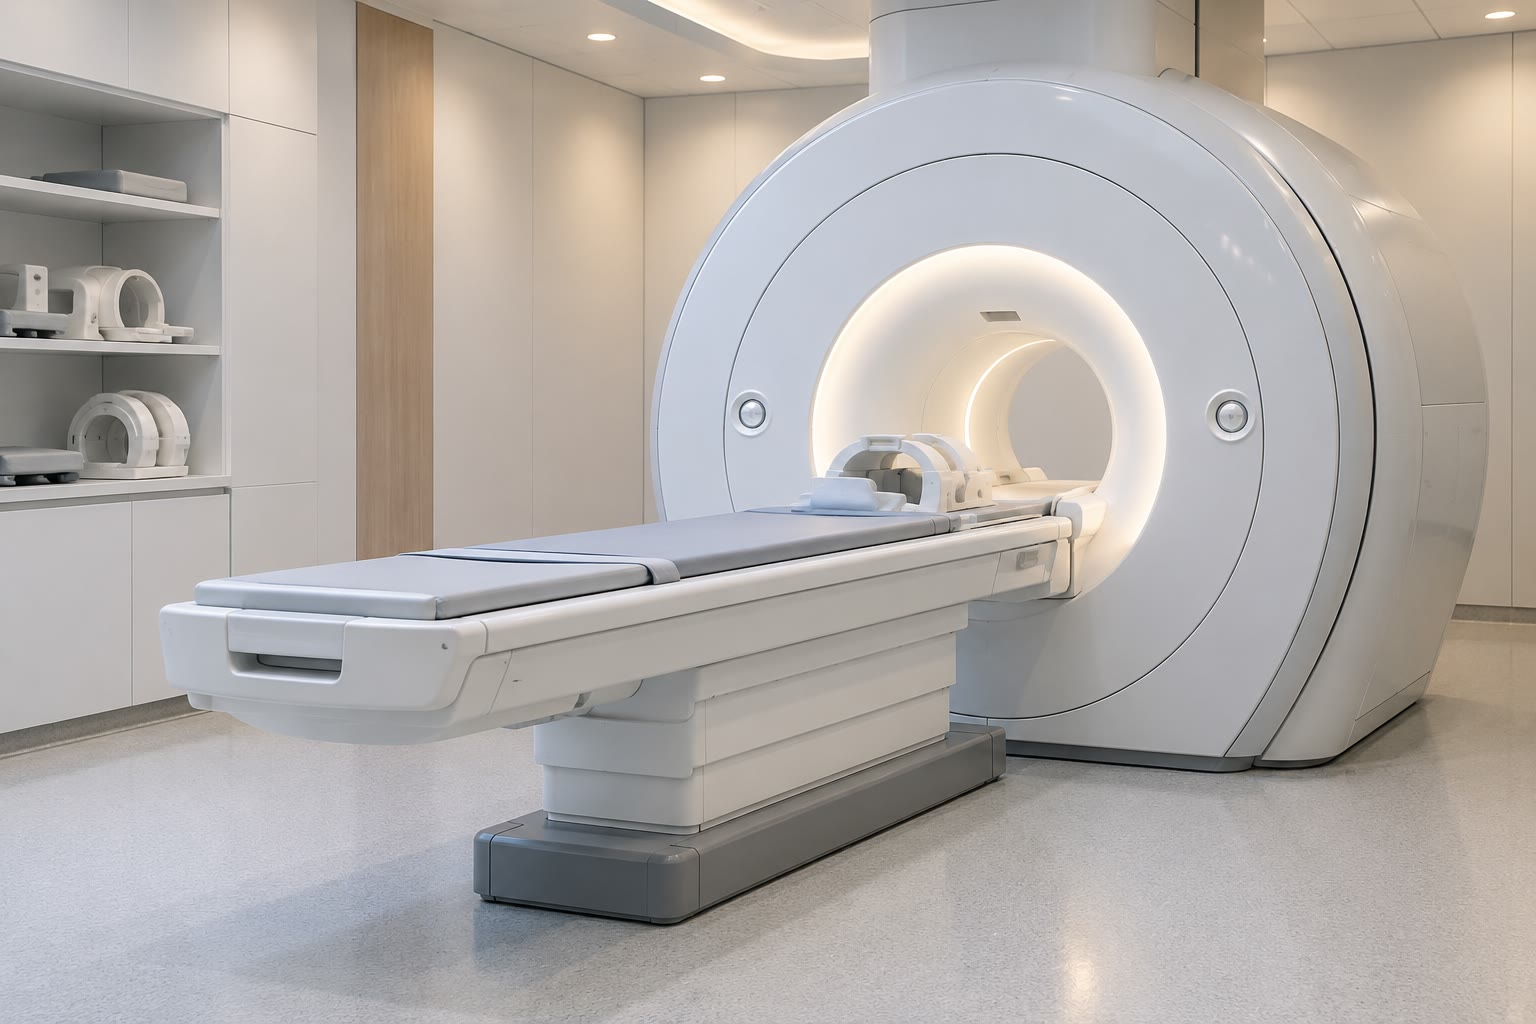
\includegraphics[width=0.52\linewidth]{images/book4/ai/b3-08-mri.jpg}\hspace{0.8em}%
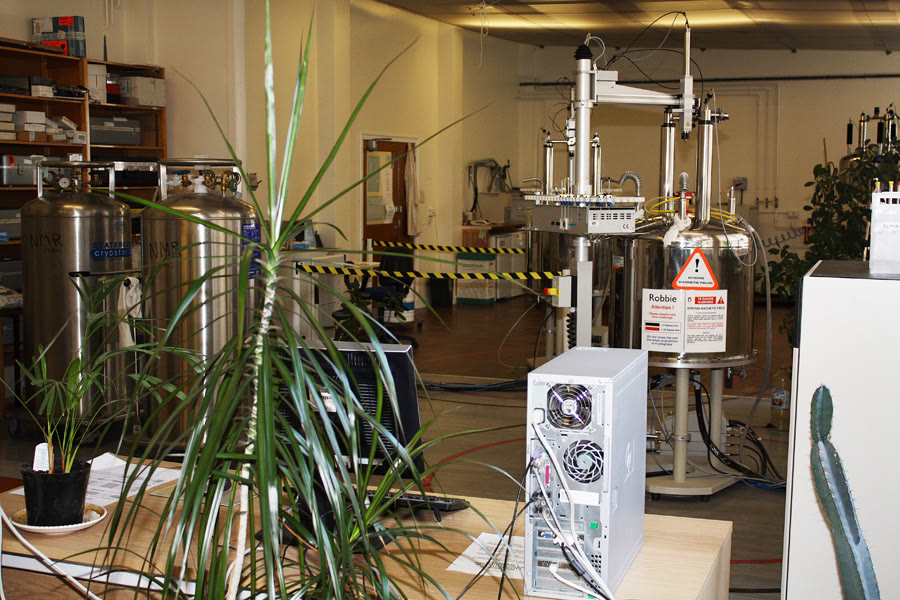
\includegraphics[width=0.4\linewidth]{images/book4/nmr-lab.jpg}

{\small À gauche~: un appareil d'IRM hospitalier. À droite~: un
laboratoire de RMN~; chaque aimant supraconducteur se tient dans son
cryostat, rempli d'hélium et d'azote liquides à partir des vases Dewar
de gauche. Photographie Shandchem, CC BY 2.0.}
\end{omfigure}

\section{Spins nucléaires dans un champ magnétique}

\begin{definition}[Nombre quantique de spin nucléaire, rapport gyromagnétique]\label{def:b3:advanced-nmr:nuclear-spin}
Un noyau possède un moment cinétique de spin de nombre quantique $I$,
son \emph{nombre quantique de spin nucléaire}\index{nombre quantique de spin nucleaire@nombre quantique de spin nucléaire} ($I = 0$
pour \ce{^{12}C}, \ce{^{16}O}~; $\frac12$ pour \ce{^1H}, \ce{^{13}C}, \ce{^{15}N}, \ce{^{19}F},
\ce{^{31}P}~; 1 pour \ce{^2H}, \ce{^{14}N}), et un moment magnétique $\boldsymbol\mu = \gamma\hat{\mathbf
I}$ qui lui est proportionnel~; $\gamma$ est le \emph{rapport gyromagnétique}\index{rapport gyromagnetique@rapport gyromagnétique}.
Selon un champ $B_0$ (axe $z$), $\hat I_z$ prend les valeurs $m_I\hbar$,
$m_I = -I, \dots, I$.
\end{definition}

\begin{proposition}[Niveaux Zeeman]\label{prop:b3:advanced-nmr:zeeman}
Dans un champ $B_0$, les niveaux sont $E_m = -m_I\gamma\hbar B_0$~; les
transitions $\Delta m_I = \pm1$
absorbent à la fréquence
\[
\nu_0 = \frac{\gamma B_0}{2\pi}.
\]
\end{proposition}

\begin{proof}
$E = -\boldsymbol\mu\cdot\mathbf B = -\gamma B_0\hat I_z$, de \omterm{def:b3:quantum-model-systems:operator}{valeurs
propres} $-\gamma B_0m_I\hbar$. Deux niveaux adjacents
diffèrent de $\gamma\hbar B_0 = h\nu_0$.
\end{proof}

\begin{definition}[Fréquence de Larmor]\label{def:b3:advanced-nmr:larmor}
$\nu_0 = \gamma B_0/2\pi$ est la \emph{fréquence de Larmor}\index{frequence de Larmor@fréquence de Larmor} du
noyau~: la fréquence de la résonance, et aussi la fréquence à laquelle
son moment magnétique précesse autour du champ.
\end{definition}

\begin{example}[Les noyaux courants]\label{ex:b3:advanced-nmr:nuclei}
% ledger: const:gammaP, nuc:C13.mu, nuc:F19.mu, nuc:P31.mu, nuc:N15.mu, const:muN
Pour un noyau de spin $\frac12$ et de moment $\mu$, $\gamma/2\pi = \mu/(Ih) = 2\mu/h$.
Avec les moments mesurés~: \ce{^1H} \qty{42.58}{MHz/T}, \ce{^{19}F} \qty{40.08}{MHz/T}, \ce{^{31}P}
\qty{17.25}{MHz/T}, \ce{^{13}C} \qty{10.71}{MHz/T}, \ce{^{15}N} \qty{-4.32}{MHz/T}. Un
«~spectromètre à \qty{400}{MHz}~» a $B_0 = \qty{9.4}{T}$~: ses protons
résonnent à
\qty{400.2}{MHz}, ses carbones à \qty{100.7}{MHz}.
\end{example}

\begin{proposition}[Une infime différence de population]\label{prop:b3:advanced-nmr:populations}
Pour un spin $\frac12$ à la température $T$, l'excès de noyaux dans le
niveau inférieur vaut
\[
\frac{N_\alpha - N_\beta}{N} \approx \frac{\gamma\hbar B_0}{2kT}.
\]
\end{proposition}

\begin{proof}
$N_\beta/N_\alpha = \eu^{-\Delta E/kT} \approx 1 - \Delta E/kT$ puisque $\Delta E \ll kT$~; donc
$(N_\alpha - N_\beta)/(N_\alpha + N_\beta) \approx \Delta E/2kT$, avec $\Delta E = \gamma\hbar B_0$.
\end{proof}

Pour des protons à \qty{9.4}{T} et \qty{300}{K}, l'excès vaut
\num{3.2e-5}~: seuls trois noyaux sur cent mille contribuent. Comme
l'excès et la tension induite dans la bobine croissent tous deux avec
$\gamma$ et $B_0$, le signal croît à peu près comme $\gamma^3B_0^2$~: d'où
la course à des aimants toujours plus intenses, et la faible sensibilité
des noyaux de petit $\gamma$ et de faible abondance naturelle, comme
\ce{^{13}C}.

\section{Impulsions et signal de précession libre}

\begin{definition}[Aimantation résultante, référentiel tournant]\label{def:b3:advanced-nmr:magnetisation}
L'\emph{aimantation résultante}\index{aimantation resultante@aimantation résultante} $\mathbf M$ d'un
échantillon est la somme de ses moments magnétiques nucléaires par unité
de volume~; à l'équilibre, elle vaut
$M_0$ selon $\mathbf B_0$. Le \emph{référentiel tournant}\index{referentiel tournant@référentiel tournant}
est un système d'axes $x'$, $y'$, $z$ tournant autour de $z$ à la
fréquence des ondes radio appliquées~; on y voit la précession à
$\nu_0$ ralentie jusqu'au décalage $\nu_0 -
\nu_{\mathrm{rf}}$.
\end{definition}

\begin{proposition}[Précession]\label{prop:b3:advanced-nmr:precession}
Une aimantation dans un champ obéit à $\dd\mathbf M/\dd t = \gamma\,\mathbf M\times\mathbf B$~;
dans un champ statique $B_0\mathbf e_z$, sa composante transversale tourne
autour de $z$ à la pulsation
$\omega_0 = \gamma B_0$, tandis que $M_z$ reste constante.
\end{proposition}

\begin{proof}[Démonstration partielle]
L'équation est l'équation classique du couple pour un moment magnétique
porteur d'un moment cinétique, admise de la physique. Avec
$\mathbf B = B_0\mathbf e_z$~: $\dot M_x = \gamma
B_0M_y$, $\dot M_y = -\gamma B_0M_x$, $\dot M_z = 0$, dont la solution est $M_x + \iu M_y \propto
\eu^{-\iu\gamma B_0t}$~: une rotation à $\omega_0$ (dans le sens horaire
vu depuis $+z$ pour $\gamma > 0$).
\end{proof}

\begin{definition}[Impulsion de radiofréquence, angle de basculement]\label{def:b3:advanced-nmr:pulse}
Une \emph{impulsion de radiofréquence}\index{impulsion de radiofrequence@impulsion de radiofréquence} est une
brève salve d'ondes radio à $\nu_{\mathrm{rf}} \approx \nu_0$, dont le
champ magnétique $B_1$, fixe dans le \omterm{def:b3:advanced-nmr:magnetisation}{référentiel tournant} selon $x'$,
fait tourner $\mathbf M$ autour de $x'$. L'angle parcouru est
l'\emph{angle de basculement}\index{angle de basculement} $\theta = \gamma B_1t_p$
pour une impulsion de durée
$t_p$~: une impulsion de $90^\circ$ amène $\mathbf M$ dans le plan $x'y'$,
une impulsion de $180^\circ$ l'inverse.
\end{definition}

\begin{omfigure}
\tdplotsetmaincoords{70}{120}
\begin{tikzpicture}[tdplot_main_coords, font=\small, >=Stealth]
  \begin{scope}
    \draw[->, gray] (0,0,0) -- (1.8,0,0) node[anchor=north east] {$x'$};
    \draw[->, gray] (0,0,0) -- (0,1.8,0) node[anchor=north west] {$y'$};
    \draw[->, gray] (0,0,0) -- (0,0,1.8) node[anchor=south] {$z$, $\mathbf B_0$};
    \draw[->, omThm, very thick] (0,0,0) -- (0,0,1.4) node[anchor=west] {$\mathbf M$};
    \node[anchor=north] at (0,0,-0.9) {équilibre};
  \end{scope}
  \begin{scope}[shift={(0,4.6,0)}]
    \draw[->, gray] (0,0,0) -- (1.8,0,0) node[anchor=north east] {$x'$};
    \draw[->, gray] (0,0,0) -- (0,1.8,0) node[anchor=north west] {$y'$};
    \draw[->, gray] (0,0,0) -- (0,0,1.8) node[anchor=south] {$z$};
    \draw[->, omDef, thick] (0,0,0) -- (1.2,0,0) node[anchor=south east, xshift=-2pt] {$\mathbf B_1$};
    \draw[->, omThm, very thick] (0,0,0) -- (0,1.4,0) node[anchor=south west] {$\mathbf M$};
    \node[anchor=north] at (0,0,-0.9) {après une impulsion $90^\circ_{x'}$};
  \end{scope}
  \begin{scope}[shift={(0,9.2,0)}]
    \draw[->, gray] (0,0,0) -- (1.8,0,0) node[anchor=north east] {$x'$};
    \draw[->, gray] (0,0,0) -- (0,1.8,0) node[anchor=north west] {$y'$};
    \draw[->, gray] (0,0,0) -- (0,0,1.8) node[anchor=south] {$z$};
    \draw[->, omThm, very thick] (0,0,0) -- (0,0,-1.4) node[anchor=west] {$\mathbf M$};
    \node[anchor=north] at (0,0,-1.6) {après une impulsion $180^\circ_{x'}$};
  \end{scope}
\end{tikzpicture}

{\small L'aimantation dans le \omterm{def:b3:advanced-nmr:magnetisation}{référentiel tournant}. Une impulsion de
$90^\circ$ autour de $x'$ fait passer $\mathbf M$ de $z$ à $y'$ (pour
$\gamma > 0$, la rotation suit la règle de la main gauche autour de
$\mathbf B_1$, convention usuelle)~; une impulsion de $180^\circ$
l'inverse.}
\end{omfigure}

\begin{definition}[Signal de précession libre]\label{def:b3:advanced-nmr:fid}
Après une impulsion de $90^\circ$, l'aimantation transversale précesse à
la \omterm{def:b3:advanced-nmr:larmor}{fréquence de Larmor} et induit une tension oscillante dans la bobine
qui entoure l'échantillon, tension qui s'éteint à mesure que
l'aimantation relaxe~: c'est le \emph{signal de précession
libre}\index{signal de precession libre@signal de précession libre} (FID).
\end{definition}

\begin{theorem}[Du FID au spectre]\label{thm:b3:advanced-nmr:lorentzian}
La transformée de Fourier d'une oscillation amortie $\eu^{-t/T_2}\cos(2\pi\nu t)$ ($t \ge 0$) est,
au voisinage de $\nu$, une raie lorentzienne de largeur à mi-hauteur
$1/(\pi T_2)$.
\end{theorem}

\begin{proof}
Écrivons le signal $\eu^{-t/T_2}\eu^{2\pi\iu\nu t}$ et intégrons~:
$\int_0^\infty\eu^{-t/T_2}\eu^{2\pi\iu(\nu - f)t}\dd t = \frac{1}{1/T_2 - 2\pi\iu(\nu - f)}$,
dont la partie réelle vaut $\frac{T_2}{1 + 4\pi^2T_2^2(f - \nu)^2}$. Elle
est maximale en $f = \nu$ et tombe à la moitié quand
$2\pi T_2|f - \nu| = 1$, c'est-à-dire en $f - \nu = \pm1/(2\pi T_2)$~:
une largeur totale de
$1/(\pi T_2)$.
\end{proof}

\begin{omfigure}
\begin{tikzpicture}
\begin{axis}[name=fid, width=0.5\linewidth, height=4.6cm, xmin=0, xmax=0.4,
  ymin=-2.1, ymax=2.1, axis lines=left, xlabel={$t$ / s}, ylabel={signal},
  ytick=\empty, scaled x ticks=false, xticklabel style={/pgf/number format/fixed},
  tick label style={font=\small}, label style={font=\small}, title={\small FID}]
\addplot[omDef] table[x=t, y=s] {figdata/out/bachelor-3-nmr-fid.dat};
\addplot[gray, dashed, domain=0:0.4, samples=60] {2*exp(-x/0.1)};
\end{axis}
\begin{axis}[at={(fid.east)}, anchor=west, xshift=1.2cm, width=0.45\linewidth,
  height=4.6cm, xmin=0, xmax=350, ymin=-0.1, ymax=1.1, axis x line=bottom,
  axis y line=none, xlabel={décalage / Hz}, tick label style={font=\small},
  label style={font=\small}, title={\small spectre (transformée de Fourier)}]
\addplot[omThm, thick] table[x=f, y=I] {figdata/out/bachelor-3-nmr-fid-spectrum.dat};
\end{axis}
\end{tikzpicture}

{\small À gauche~: le FID de deux raies (décalages de 100 et de
\qty{250}{Hz}, $T_2 = \qty{0.10}{s}$), présentant des battements dus à
l'interférence des deux fréquences dans une enveloppe exponentielle (en
tirets). À droite~: sa transformée de Fourier, deux raies lorentziennes
larges de \qty{3.2}{Hz}.}
\end{omfigure}

\begin{proposition}[Accumulation du signal]\label{prop:b3:advanced-nmr:averaging}
Additionner $N$ FID multiplie le signal par $N$ et le bruit aléatoire par
$\sqrt N$~: le rapport signal sur bruit croît comme $\sqrt N$.
\end{proposition}

\begin{proof}
Le signal s'additionne de façon cohérente. Le bruit d'acquisitions
indépendantes est de moyenne nulle et de variance $\sigma^2$ chacune~; la
variance d'une somme de $N$ termes indépendants vaut
$N\sigma^2$ (la loi de propagation du volume de deuxième année), donc son
écart-type vaut $\sqrt N\sigma$.
\end{proof}

Le DEPT, qui trie les signaux de ${}^{13}$C selon le nombre d'hydrogènes
portés, applique aux protons et aux carbones une séquence d'impulsions
séparées par des délais de $1/2J$~: la grande aimantation des protons est
transférée au carbone par le couplage à une liaison, ce qui multiplie le
signal du carbone par environ
$\gamma_H/\gamma_C \approx 4$, et l'angle de la dernière impulsion sur
les protons pondère différemment CH, \ce{CH2} et
\ce{CH3}. La même idée --- déplacer l'aimantation d'un noyau à l'autre par
leurs couplages --- sous-tend les expériences bidimensionnelles
ci-dessous.

\section{Relaxation}

\begin{definition}[Temps de relaxation longitudinale et transversale]\label{def:b3:advanced-nmr:relaxation}
Le retour de $M_z$ à $M_0$ après une perturbation est exponentiel, avec
le \emph{temps de relaxation longitudinale}\index{temps de relaxation longitudinale} $T_1$
(relaxation spin--réseau~: énergie cédée au milieu). La décroissance de
l'aimantation transversale jusqu'à zéro est exponentielle, avec le
\emph{temps de relaxation transversale}\index{temps de relaxation transversale} $T_2 \le T_1$
(relaxation spin--spin~: perte de cohérence de phase entre les spins).
\end{definition}

\begin{proposition}[Inversion-récupération]\label{prop:b3:advanced-nmr:inversion-recovery}
Après une impulsion de $180^\circ$, $M_z(t) = M_0(1 - 2\eu^{-t/T_1})$~;
elle s'annule en
$t_{\mathrm{null}} = T_1\ln2$.
\end{proposition}

\begin{proof}
L'équation de relaxation $\dd M_z/\dd t = (M_0 - M_z)/T_1$ avec $M_z(0) = -M_0$ a pour
solution $M_0 - 2M_0\eu^{-t/T_1}$, qui s'annule quand $\eu^{-t/T_1} = \frac12$.
\end{proof}

\begin{method}[Mesurer $T_1$ et régler un délai de recyclage quantitatif]\label{met:b3:advanced-nmr:t1}
\begin{enumerate}
  \item Appliquer la séquence $180^\circ$--$\tau$--$90^\circ$--acquisition
        pour une série de délais
        $\tau$, en attendant au moins $5T_1$ entre deux acquisitions.
  \item Ajuster chaque signal sur $M_0(1 - 2\eu^{-\tau/T_1})$, ou lire le
        passage à zéro~: $T_1 =
        t_{\mathrm{null}}/\ln2$.
  \item Pour une intégration quantitative avec des impulsions de
        $90^\circ$, attendre au moins $5T_1$ du noyau le plus lent entre
        deux acquisitions~: il manque alors moins de $\eu^{-5} < 1\,\%$
        de l'aimantation.
\end{enumerate}
\end{method}

\begin{omfigure}
\begin{tikzpicture}
\begin{axis}[width=0.62\linewidth, height=5cm, xmin=0, xmax=10, ymin=-1.1, ymax=1.15,
  axis lines=left, xlabel={$t$ / s}, ylabel={$M/M_0$}, legend cell align=left,
  legend style={font=\small, draw=none, at={(0.97,0.05)}, anchor=south east},
  tick label style={font=\small}, label style={font=\small}]
\addplot[omDef, thick] table[x=t, y=mz] {figdata/out/bachelor-3-nmr-relaxation.dat};
\addlegendentry{$M_z$ après $180^\circ$ ($T_1 = \qty{2.0}{s}$)}
\addplot[omThm, thick, dashed] table[x=t, y=mxy] {figdata/out/bachelor-3-nmr-relaxation.dat};
\addlegendentry{$M_{xy}$ après $90^\circ$ ($T_2 = \qty{0.5}{s}$)}
\addplot[gray, dotted, domain=0:10] {0};
\addplot[only marks, mark=*, mark size=1.5pt, black] coordinates {(1.386,0)};
\node[font=\small, anchor=north west] at (axis cs:1.5,-0.04) {$T_1\ln2$};
\end{axis}
\end{tikzpicture}

{\small Relaxation (valeurs modèles). L'aimantation longitudinale inversée
revient en passant par zéro à $T_1\ln2$~; l'aimantation transversale
décroît plus vite, avec $T_2$.}
\end{omfigure}

\begin{definition}[Écho de spin]\label{def:b3:advanced-nmr:echo}
Dans la séquence $90^\circ$--$\tau$--$180^\circ$--$\tau$, les spins qui se
sont déphasés à cause des inhomogénéités du champ sont refocalisés au
temps $2\tau$, ce qui produit un
\emph{écho de spin}\index{echo de spin@écho de spin}~; son amplitude
décroît avec le vrai $T_2$, affranchie de
l'inhomogénéité de l'aimant.
\end{definition}

\begin{definition}[Effet Overhauser nucléaire]\label{def:b3:advanced-nmr:noe}
Saturer ou perturber un spin modifie, par leur relaxation dipolaire,
l'intensité du signal d'un autre spin proche dans l'espace~: c'est
l'\emph{effet Overhauser nucléaire}\index{effet Overhauser nucleaire@effet Overhauser nucléaire} (NOE).
Sa vitesse d'établissement est proportionnelle à $r^{-6}$, si bien qu'on
ne l'observe qu'entre noyaux distants de moins d'environ \qty{0.5}{nm},
qu'ils soient liés ou non.
\end{definition}

\section{La RMN bidimensionnelle}

\begin{definition}[Spectre bidimensionnel, pic de corrélation, pic diagonal]\label{def:b3:advanced-nmr:two-d}
Un \emph{spectre bidimensionnel}\index{spectre bidimensionnel} s'enregistre
en répétant une séquence d'impulsions avec un délai $t_1$ incrémenté
avant le temps d'acquisition $t_2$~; une double transformée de Fourier
donne une carte de l'intensité en fonction de deux fréquences. Un
\emph{pic de corrélation}\index{pic de correlation@pic de corrélation} en $(\delta_1,
\delta_2)$ montre que les noyaux à $\delta_1$ et à $\delta_2$ sont reliés
(par un couplage ou par la proximité)~; un \emph{pic
diagonal}\index{pic diagonal} en $(\delta, \delta)$ appartient à un seul
noyau.
\end{definition}

\begin{definition}[COSY, HSQC, HMBC, NOESY]\label{def:b3:advanced-nmr:experiments}
La \emph{COSY}\index{COSY} (spectroscopie de corrélation) corrèle des
protons couplés entre eux, en général à travers trois liaisons
(H--C--C--H). La \emph{HSQC}\index{HSQC}
(cohérence hétéronucléaire à un quantum) corrèle chaque carbone avec les
protons qui lui sont directement liés. La \emph{HMBC}\index{HMBC}
(corrélation hétéronucléaire à plusieurs liaisons) corrèle des carbones
avec des protons distants de deux ou trois liaisons, par-delà les
carbones quaternaires et les hétéroatomes. La \emph{NOESY}\index{NOESY}
corrèle des protons proches dans l'espace par l'\omterm{def:b3:advanced-nmr:noe}{effet Overhauser
nucléaire}.
\end{definition}

\begin{omfigure}
\begin{tikzpicture}[font=\small]
  \foreach \y/\name in {3.2/{une impulsion}, 2.0/{inversion-récupération}, 0.8/{écho de spin}, -0.4/{COSY}}{
    \draw (0,\y) -- (9.3,\y); \node[anchor=east] at (-0.1,\y+0.25) {\name};}
  % one pulse
  \fill[black] (0.4,3.2) rectangle (0.6,3.75);
  \draw[omDef, domain=0:3.5, samples=120] plot (0.7+\x, {3.2+0.4*exp(-\x/1.2)*sin(\x*500)});
  % inversion recovery
  \fill[black] (0.4,2.0) rectangle (0.8,2.55); \node[font=\scriptsize] at (0.6,2.7) {180};
  \draw[<->] (0.85,1.85) -- (2.4,1.85) node[midway, below, font=\scriptsize] {$\tau$};
  \fill[black] (2.45,2.0) rectangle (2.65,2.55); \node[font=\scriptsize] at (2.55,2.7) {90};
  \draw[omDef, domain=0:3.0, samples=120] plot (2.75+\x, {2.0+0.4*exp(-\x/1.0)*sin(\x*500)});
  % spin echo
  \fill[black] (0.4,0.8) rectangle (0.6,1.35); \node[font=\scriptsize] at (0.5,1.5) {90};
  \draw[<->] (0.65,0.65) -- (2.4,0.65) node[midway, below, font=\scriptsize] {$\tau$};
  \fill[black] (2.45,0.8) rectangle (2.85,1.35); \node[font=\scriptsize] at (2.65,1.5) {180};
  \draw[<->] (2.9,0.65) -- (4.65,0.65) node[midway, below, font=\scriptsize] {$\tau$};
  \draw[omDef, domain=-1.2:2.5, samples=150] plot (4.65+\x, {0.8+0.35*exp(-abs(\x)/0.35)*cos(\x*700)});
  % COSY
  \fill[black] (0.4,-0.4) rectangle (0.6,0.15); \node[font=\scriptsize] at (0.5,0.3) {90};
  \draw[<->] (0.65,-0.55) -- (2.4,-0.55) node[midway, below, font=\scriptsize] {$t_1$ (incrémenté)};
  \fill[black] (2.45,-0.4) rectangle (2.65,0.15); \node[font=\scriptsize] at (2.55,0.3) {90};
  \draw[omDef, domain=0:3.0, samples=120] plot (2.75+\x, {-0.4+0.4*exp(-\x/1.0)*sin(\x*500)});
  \node[font=\scriptsize, anchor=west] at (5.9,-0.2) {acquisition ($t_2$)};
\end{tikzpicture}

{\small Séquences d'impulsions (le temps croît vers la droite~; rectangles
pleins~: impulsions, repérées par leur \omterm{def:b3:advanced-nmr:pulse}{angle de basculement} en degrés~;
bleu~: le signal enregistré). L'\omterm{def:b3:advanced-nmr:echo}{écho de spin} culmine à $2\tau$ après la
première impulsion.}
\end{omfigure}

\begin{method}[Résoudre une structure à l'aide de spectres bidimensionnels]\label{met:b3:advanced-nmr:solve-2d}
\begin{enumerate}
  \item À partir de la formule brute, des intégrales en ${}^1$H et du
        spectre de ${}^{13}$C/DEPT, dresser la liste
        des carbones CH, \ce{CH2}, \ce{CH3} et quaternaires.
  \item \omterm{def:b3:advanced-nmr:experiments}{HSQC}~: rattacher chaque signal de proton à son carbone.
  \item \omterm{def:b3:advanced-nmr:experiments}{COSY}~: réunir les carbones protonés en systèmes de spins (chaînes
        de voisins).
  \item \omterm{def:b3:advanced-nmr:experiments}{HMBC}~: relier les systèmes de spins par-delà les carbones
        quaternaires, les carbonyles et les hétéroatomes, là où la \omterm{def:b3:advanced-nmr:experiments}{COSY}
        est muette.
  \item \omterm{def:b3:advanced-nmr:experiments}{NOESY}~: fixer les configurations relatives et les conformations
        à partir des contacts à travers l'espace.
  \item Confronter chaque signal à la structure proposée.
\end{enumerate}
\end{method}

\begin{omfigure}
\begin{tikzpicture}
\begin{axis}[name=cosy, width=0.47\linewidth, height=0.47\linewidth, x dir=reverse,
  y dir=reverse, xmin=0.5, xmax=4.6, ymin=0.5, ymax=4.6, axis lines=box,
  xlabel={$\delta_{\mathrm H}$ / ppm}, ylabel={$\delta_{\mathrm H}$ / ppm},
  tick label style={font=\small}, label style={font=\small}, title={\small COSY}]
\addplot[gray, dotted, domain=0.5:4.6] {x};
\addplot[only marks, mark=*, mark size=2.2pt, black] table[x=h1, y=h2] {figdata/out/bachelor-3-nmr-2d-cosy-diag.dat};
\addplot[only marks, mark=*, mark size=2.2pt, omThm] table[x=h1, y=h2] {figdata/out/bachelor-3-nmr-2d-cosy-cross.dat};
\end{axis}
\begin{axis}[at={(cosy.east)}, anchor=west, xshift=1.3cm, width=0.47\linewidth,
  height=0.47\linewidth, x dir=reverse, y dir=reverse, xmin=0.5, xmax=4.6,
  ymin=0, ymax=185, axis lines=box, xlabel={$\delta_{\mathrm H}$ / ppm},
  ylabel={$\delta_{\mathrm C}$ / ppm}, tick label style={font=\small},
  label style={font=\small}, title={\small HSQC (bleu) et HMBC (rouge)}]
\addplot[only marks, mark=square*, mark size=2.2pt, omDef] table[x=h, y=c] {figdata/out/bachelor-3-nmr-2d-hsqc.dat};
\addplot[only marks, mark=o, mark size=2.6pt, omThm, thick] table[x=h, y=c] {figdata/out/bachelor-3-nmr-2d-hmbc.dat};
\end{axis}
\end{tikzpicture}

{\small \omterm{def:b3:advanced-nmr:two-d}{Spectres bidimensionnels} du butanoate d'éthyle,
\ce{CH3CH2CH2COOCH2CH3}, tracés à ses déplacements mesurés. \omterm{def:b3:advanced-nmr:experiments}{COSY}~: en
noir, les pics diagonaux~; en rouge, les \omterm{def:b3:advanced-nmr:two-d}{pics de corrélation} entre
protons portés par des carbones voisins --- deux systèmes de spins,
éthyle et propyle, sans \omterm{def:b3:advanced-nmr:two-d}{pic de corrélation} à travers l'oxygène de l'ester.
À droite~: les pics \omterm{def:b3:advanced-nmr:experiments}{HSQC}
(carrés) relient chaque proton à son carbone~; les pics \omterm{def:b3:advanced-nmr:experiments}{HMBC} (cercles)
montrent que les protons OCH$_2$
(\qty{4.13}{ppm}) et les protons CH$_2$C=O (\qty{2.28}{ppm}) atteignent
tous deux le carbone du carbonyle à \qty{173.6}{ppm}.}
\end{omfigure}

\section{Autres noyaux et dynamique}

Le fluor 19 et le phosphore 31, de spin $\frac12$, abondants à 100\,\% et
de grand
$\gamma$, s'observent presque aussi facilement que les protons~; leurs
larges gammes de déplacements en font des sondes précises de leur
environnement (médicaments, phosphates, ligands comme les phosphines du
\cref{ch:b3:organometallic-bonding}). L'azote 15 est rare et peu
sensible~; on l'observe en général indirectement, par les protons qui
lui sont liés. Le couplage entre noyaux différents est supprimé par
découplage, comme pour le ${}^{13}$C dans le volume de deuxième année.

\begin{definition}[Température de coalescence]\label{def:b3:advanced-nmr:coalescence}
Quand un noyau s'échange entre deux environnements dont les déplacements
sont séparés de $\Delta\nu$ (en hertz), ses deux raies s'élargissent à
mesure que l'échange s'accélère et fusionnent en une seule à la
\emph{température de coalescence}\index{temperature de coalescence@température de coalescence}
$T_c$.
\end{definition}

\begin{proposition}[Vitesse à la coalescence]\label{prop:b3:advanced-nmr:coalescence}
Pour deux sites également peuplés et sans couplage, la constante de
vitesse d'échange à la coalescence vaut $k_c = \pi\Delta\nu/\sqrt2$.
\end{proposition}
\admitted

La démonstration, à partir des équations de Bloch avec échange, relève de
cours plus avancés. Avec l'équation d'Eyring (\cref{ch:b3:rate-theories}),
la vitesse donne la barrière~: la RMN dynamique mesure les rotations
autour des liaisons amide, les inversions de cycle et les échanges de
ligands, de barrières comprises entre 40 et \qty{100}{kJ/mol}.

\begin{example}[Une image d'IRM]\label{ex:b3:advanced-nmr:mri}
En imagerie par résonance magnétique, un gradient de champ rend la
\omterm{def:b3:advanced-nmr:larmor}{fréquence de Larmor} des protons de l'eau dépendante de la position, si
bien que la transformée de Fourier du signal est une carte de leur
répartition. Le contraste vient de la relaxation~: on choisit le temps de
répétition et les délais d'écho pour pondérer l'image en $T_1$ ou en
$T_2$, qui diffèrent d'un tissu à l'autre~; les agents de contraste au
gadolinium raccourcissent le $T_1$ de l'eau voisine
(\cref{ch:b3:bioinorganic}).
\end{example}

\begin{inthelab}[Préparer un spectromètre]
L'échantillon, dissous dans un solvant deutéré, descend dans la sonde. Le
spectromètre se verrouille sur le signal du deutérium pour compenser la
lente dérive du champ~; la sonde est accordée et adaptée à la fréquence
de chaque noyau~; le champ est rendu homogène sur l'échantillon en
réglant les bobines de correction (shims) jusqu'à ce que les raies
soient fines. Le champ de l'aimant est permanent~: outils en acier,
cartes bancaires et stimulateurs cardiaques restent en dehors de la
ligne de sécurité tracée au sol.
\end{inthelab}

\begin{history}[De la résonance aux deux dimensions]
Felix Bloch et Edward Purcell détectèrent la résonance magnétique
nucléaire dans la matière condensée en 1946 (prix Nobel de physique
1952). Richard Ernst introduisit la RMN impulsionnelle par transformée de
Fourier en 1966 puis, à partir d'une idée de Jean Jeener, la
spectroscopie bidimensionnelle dans les années 1970 (prix Nobel de
chimie 1991).
\end{history}

\section{Exercices}

\begin{exercise}[$\star$]\label{exo:b3:advanced-nmr:1}
% ledger: const:gammaP, nuc:C13.mu, nuc:F19.mu
Calculer les \omterm{def:b3:advanced-nmr:larmor}{fréquences de Larmor} de \ce{^1H}, \ce{^{13}C} et \ce{^{19}F}
à \qty{14.1}{T}
($\gamma/2\pi = 42.58$, 10.71 et \qty{40.08}{MHz/T}).
\end{exercise}

\begin{exercise}[$\star$]\label{exo:b3:advanced-nmr:2}
Calculer l'excès relatif de protons dans le niveau inférieur à
\qty{9.4}{T} et
\qty{300}{K}. Comment change-t-il à \qty{4}{K}~?
\end{exercise}

\begin{exercise}[$\star$]\label{exo:b3:advanced-nmr:3}
Une impulsion de $90^\circ$ dure \qty{10}{\micro s} pour les protons.
Que vaut $\gamma B_1/2\pi$~? Combien dure une impulsion de
$180^\circ$, et que fait une impulsion de \qty{5}{\micro s}~?
\end{exercise}

\begin{exercise}[$\star$]\label{exo:b3:advanced-nmr:4}
Une raie a une largeur à mi-hauteur de \qty{3.2}{Hz}. Que vaut $T_2$ (en
supposant le champ parfaitement homogène)~?
\end{exercise}

\begin{exercise}[$\star\star$]\label{exo:b3:advanced-nmr:5}
% ledger: iso:C13
En prenant un signal $\propto\gamma^3$ par noyau et l'abondance naturelle
de 1.1\,\% du
\ce{^{13}C}, comparer les sensibilités des RMN du ${}^{13}$C et du
${}^1$H. Combien d'acquisitions supplémentaires un spectre de ${}^{13}$C
exige-t-il pour le même rapport signal sur bruit~?
\end{exercise}

\begin{exercise}[$\star\star$]\label{exo:b3:advanced-nmr:6}
Dans une expérience d'inversion-récupération, le signal d'un carbone
s'annule pour
$\tau = \qty{1.39}{s}$. Trouver $T_1$ et le délai de recyclage pour un
travail quantitatif.
\end{exercise}

\begin{exercise}[$\star\star$]\label{exo:b3:advanced-nmr:7}
Dans le spectre \omterm{def:b3:advanced-nmr:experiments}{COSY} de la butanone, \ce{CH3COCH2CH3}, quels \omterm{def:b3:advanced-nmr:two-d}{pics de
corrélation} apparaissent~? Quels carbones présentent des pics \omterm{def:b3:advanced-nmr:experiments}{HMBC} avec
les protons du méthyle singulet~?
\end{exercise}

\begin{exercise}[$\star\star$]\label{exo:b3:advanced-nmr:8}
Deux signaux de méthyle d'un amide, distants de \qty{50}{Hz} à basse
température, coalescent à
\qty{330}{K}. Calculer la vitesse d'échange à la coalescence et
l'enthalpie libre d'activation à l'aide de
$\Delta G^\ddagger = RT_c\ln(k_BT_c/hk_c)$.
\end{exercise}

\begin{exercise}[$\star\star$]\label{exo:b3:advanced-nmr:9}
Un NOE entre les protons H$_a$ et H$_b$ est quatre fois plus intense
qu'entre H$_a$ et
H$_c$, situés à \qty{0.30}{nm}. Estimer la distance H$_a$--H$_b$.
\end{exercise}

\begin{exercise}[$\star\star\star$]\label{exo:b3:advanced-nmr:10}
Montrer, en résolvant $\dd\mathbf M/\dd t = \gamma\mathbf M\times\mathbf B_1$ dans le \omterm{def:b3:advanced-nmr:magnetisation}{référentiel tournant}
avec $\mathbf B_1$ selon $x'$, qu'une impulsion fait tourner $\mathbf M$
de $\gamma B_1t_p$ autour de $x'$.
\end{exercise}

\begin{exercise}[$\star\star\star$]\label{exo:b3:advanced-nmr:11}
Expliquer pourquoi l'\omterm{def:b3:advanced-nmr:echo}{écho de spin} refocalise le déphasage dû à un champ
inhomogène, mais pas celui dû aux interactions aléatoires entre spins.
Quelle constante de temps l'amplitude de l'écho mesure-t-elle~?
\end{exercise}

\begin{exercise}[$\star\star\star$]\label{exo:b3:advanced-nmr:12}
Proposer la structure d'un composé \ce{C4H8O2} dont le spectre de
${}^1$H présente un
quadruplet (2H, 4.12 ppm), un singulet (3H, 2.05 ppm) et un triplet (3H,
1.26 ppm), et dont le spectre \omterm{def:b3:advanced-nmr:experiments}{HMBC} corrèle les protons du quadruplet
avec un carbone à 171 ppm (données de l'exercice). Quel autre ester de
même formule donnerait une figure \omterm{def:b3:advanced-nmr:experiments}{HMBC} différente, et en quoi~?
\end{exercise}

\section{Problème~: l'ester de l'ananas en deux dimensions}

\begin{problem}[{Problème du week-end --- le butanoate d'éthyle en deux
dimensions~: systèmes de spins (COSY), carbones (HSQC), liaison ester
(HMBC) et délai d'un spectre de carbone quantitatif}]
\label{pb:b3:advanced-nmr:1}
% ledger: nmr:ethylbutanoate-OCH2, nmr:ethylbutanoate-CH2CO, nmr:ethylbutanoate-CH2, nmr:ethylbutanoate-OCH2CH3, nmr:ethylbutanoate-CH3, c13:ethylbutanoate.CO, c13:ethylbutanoate.OCH2, c13:ethylbutanoate.CH2CO, c13:ethylbutanoate.CH2, c13:ethylbutanoate.OCH2CH3, c13:ethylbutanoate.CH3
Un ester \ce{C6H12O2} de l'arôme de l'ananas présente des signaux de
${}^1$H à 4.13 (2H,
q), 2.28 (2H, t), 1.66 (2H, m), 1.25 (3H, t) et 0.95 ppm (3H, t), et des
signaux de ${}^{13}$C
à 173.6, 60.1, 36.3, 18.6, 14.3 et 13.7 ppm, enregistrés à
\qty{9.4}{T}. Ses spectres 2D sont ceux de la figure de la section 4.
Données du problème~: les $T_1$
des carbones valent environ \qty{20}{s} pour le carbonyle, de 2 à
\qty{6}{s} pour les autres.

\medskip\noindent\textbf{Partie I --- Une dimension.}
\begin{enumerate}
  \item Calculer le nombre d'insaturations de \ce{C6H12O2}.
  \item Quel signal de ${}^{13}$C est le carbonyle~? Lequel est le carbone
        lié à l'oxygène~?
  \item Combien y a-t-il de carbones protonés~? Que montrerait le
        DEPT-135~?
  \item À \qty{9.4}{T}, quelles sont les \omterm{def:b3:advanced-nmr:larmor}{fréquences de Larmor} de ${}^1$H
        et de ${}^{13}$C~?
  \item Le couplage du quadruplet vaut \qty{7.2}{Hz}~: quelle est sa
        largeur, en ppm, à \qty{400}{MHz}~?
  \item Pourquoi les seuls spectres 1D peuvent-ils laisser ouvert l'ordre
        des fragments~?
\end{enumerate}

\medskip\noindent\textbf{Partie II --- \omterm{def:b3:advanced-nmr:experiments}{COSY}.}
\begin{enumerate}[resume]
  \item Énumérer les \omterm{def:b3:advanced-nmr:two-d}{pics de corrélation} de la carte \omterm{def:b3:advanced-nmr:experiments}{COSY}.
  \item En déduire les deux systèmes de spins.
  \item Pourquoi n'y a-t-il pas de \omterm{def:b3:advanced-nmr:two-d}{pic de corrélation} entre 4.13 et
        2.28 ppm~?
  \item Quel signal de proton est couplé à deux autres~? Expliquer sa
        multiplicité.
  \item Qu'aurait signifié un \omterm{def:b3:advanced-nmr:two-d}{pic de corrélation} entre 0.95 et
        1.25 ppm~?
  \item Dessiner les deux fragments.
\end{enumerate}

\medskip\noindent\textbf{Partie III --- \omterm{def:b3:advanced-nmr:experiments}{HSQC} et \omterm{def:b3:advanced-nmr:experiments}{HMBC}.}
\begin{enumerate}[resume]
  \item À partir de la \omterm{def:b3:advanced-nmr:experiments}{HSQC}, attribuer chaque carbone à ses protons.
  \item Quels deux carbones de méthyle ne sont distingués que par la
        \omterm{def:b3:advanced-nmr:experiments}{HSQC}~?
  \item Quel pic \omterm{def:b3:advanced-nmr:experiments}{HMBC} relie le fragment éthyle au carbonyle, et à travers
        combien de liaisons~?
  \item Quels pics \omterm{def:b3:advanced-nmr:experiments}{HMBC} relient le fragment propyle au carbonyle~?
  \item En déduire la structure, et exclure son isomère, le propanoate de
        propyle.
  \item Pourquoi les pics \omterm{def:b3:advanced-nmr:experiments}{HMBC} à travers quatre liaisons ou plus sont-ils
        en général absents~?
\end{enumerate}

\medskip\noindent\textbf{Partie IV --- Un spectre de carbone quantitatif.}
\begin{enumerate}[resume]
  \item Pourquoi les intégrales d'un spectre de ${}^{13}$C ordinaire ne
        sont-elles pas proportionnelles au nombre de carbones~?
  \item Quelle fraction de son aimantation d'équilibre le carbonyle
        récupère-t-il si les acquisitions sont répétées toutes les
        \qty{5}{s} avec des impulsions de $90^\circ$ (en partant chaque
        fois de zéro)~?
  \item Quelle fraction après $5T_1$~?
  \item Outre la relaxation, quel effet du découplage des protons fausse
        les intégrales des carbones, et comment le supprime-t-on~?
  \item Avec un délai de $5T_1$, combien de temps durent 256
        acquisitions~?
  \item Énoncer le résultat~: le délai de recyclage minimal pour un
        spectre de ${}^{13}$C quantitatif de cet ester.
\end{enumerate}
\end{problem}
